\documentclass{article}
\usepackage{amsmath, amssymb}
\usepackage{tikz}

\begin{document}

\section*{Illustration Of Lemma \ref{lem:herali1} in the case \( E = \mathbb{R}^2 \), with \(\varepsilon_2\) being the sinus of the angle between the main axis of the ellipse \( h(\mathbf{S}) \) and the dashed line \(\ker(w_1^g) \) on the left of the arrow with \(\varepsilon_2\) being the angle between the dotted ellipse \( g(\mathbf{S}) \) and the dashed line \(\ker(w^f_1)\) and with \(\varepsilon_3\) being the angle between the plain ellipse \( gh(\mathbf{S}) \) and the dashed line. We write \(\mathbf{S}\) for the unit sphere.}

\begin{figure}[h]
    \centering
    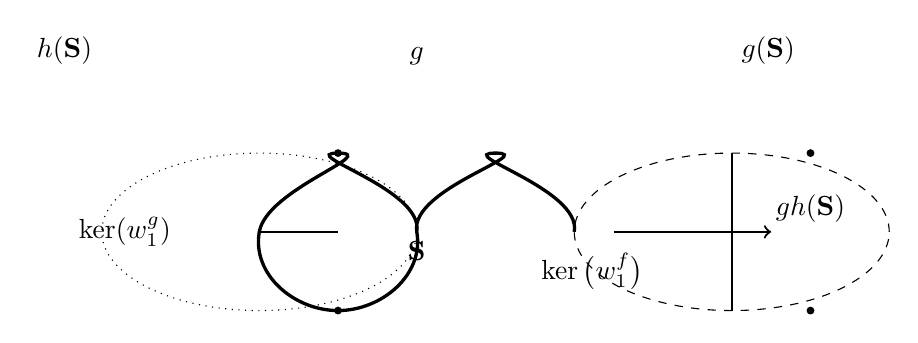
\begin{tikzpicture}
        % Ellipse 1 (left)
        \draw[dotted] (0,0) ellipse (2 and 1); % Main ellipse
        \draw[thick] (0,0) -- (1,0); % Dashed line k
        \node at (-1,0) [left] {$\ker(w_1^g)$};
        
        % Ellipse 2 (right)
        \draw[dashed] (6,0) ellipse (2 and 1); % Dotted ellipse
        \draw[thick] (6,-1) -- (6,1); % Dashed line k
        \node at (5,-0.5) [left] {$\ker\big( w^f_1 \big)$};
        
        % Plain ellipse
        \draw[very thick] (4,0) to[out=80,in=180] (3,1) to[out=0,in=100] (2,0) to[out=-80,in=0] (1,-1) to[out=180,in=-100] (0,0) to[out=80,in=0] (1,1) to[out=180,in=80] (2,0);
        \node at (7,0) [above] {$gh(\mathbf{S})$};
        
        % Labels
        \node at (1,1) [circle, fill, inner sep=1pt] {};
        \node at (1,-1) [circle, fill, inner sep=1pt] {};
        \node at (7,1) [circle, fill, inner sep=1pt] {};
        \node at (7,-1) [circle, fill, inner sep=1pt] {};
        \node at (-2,2) [above left] {$h(\mathbf{S})$};
        \node at (6,2) [above right] {$g(\mathbf{S})$};
        \node at (2,2) [above] {$g$};
        \node at (2,0) [below] {$\mathbf{S}$};
        
        % Arrows
        \draw[->, thick] (4.5,0) -- (6.5,0);
    \end{tikzpicture}
    \caption{Illustration of Lemma \ref{lem:herali1} as described.}
    \label{fig:herali1}
\end{figure}

\end{document}